\documentclass[12p]{article}

\title{\huge Wyznaczanie liczby $ \pi $}
\date{Analiza Numeryczna (M) - Zadanie P1.4\\ 22 października 2020}
\author{\Large Kacper Kingsford}

\usepackage[T1]{fontenc}
\usepackage[utf8]{inputenc}
\usepackage{lmodern}
\usepackage[margin=0.9in]{geometry}
\usepackage{amsthm}
\usepackage{amsmath}
\usepackage{tikz}
\usepackage{amsfonts} 

\makeatletter
\let\sv@endpart\@endpart
\def\@endpart{\thispagestyle{empty}\sv@endpart}
\makeatother


\usepackage{graphicx}
\graphicspath{ {/Desktop/programowanie/ANM/P1/doc/} }
\renewcommand*\contentsname{Spis treści}
\usepackage{listings}
\usepackage{xcolor}

\definecolor{codegreen}{rgb}{0,0.6,0}
\definecolor{codegray}{rgb}{0.5,0.5,0.5}
\definecolor{codepurple}{rgb}{0.58,0,0.82}
\definecolor{backcolour}{rgb}{0.95,0.95,0.92}
\usepackage{ragged2e}

\lstdefinelanguage{Julia}%
{
    morekeywords={%
        exit,whos,edit,load,is,isa,isequal,typeof,tuple,ntuple,uid,hash,finalizer,convert,promote,%
        subtype,typemin,typemax,realmin,realmax,sizeof,eps,promote_type,method_exists,applicable,%
        invoke,dlopen,dlsym,system,error,throw,assert,new,Inf,Nan,pi,im,begin,while,for,in,return,%
        break,continue,macro,quote,let,if,elseif,else,try,catch,end,bitstype,ccall,do,using,module,%
        import,export,importall,baremodule,immutable,local,global,const,Bool,Int,Int8,Int16,Int32,%
        Int64,Uint,Uint8,Uint16,Uint32,Uint64,Float32,Float64,Complex64,Complex128,Any,Nothing,None,%
        function,type,typealias,abstract%
  },%
  sensitive=true,%
  morecomment=[l]\#,%
  morecomment=[n]{\#=}{=\#},%
  morestring=[s]{"}{"},%
  morestring=[m]{'}{'},%
}[keywords, comments, strings]%

\lstset{%
    language         = Julia,
    basicstyle       = \ttfamily,
    keywordstyle     = \bfseries\color{blue},
    columns          = fullflexible,
    stringstyle      = \color{magenta},
    commentstyle     = \color{gray},
    showstringspaces = false,
    numbers          = left,
    xleftmargin      = 2em
}


\begin{document}
\begin{titlepage}

\maketitle
\thispagestyle{empty}
\begin{center}
	\textbf{\large Streszczenie}
\end{center}
\par Liczba $\pi$ (zwana inaczej ludolfiną) jest jedną z pierwszych odkrytych przez człowieka liczb niewymiernych. Oznacza stosunek długości obwodu koła do długości jego średnicy. Jest też pierwszą literą greckiego słowa "perimetron”, oznaczającego obwód. Datę 14 marca na Dzień Liczby Pi wybrano nieprzypadkowo - w Stanach Zjednoczonych zapisuje się ją jako $3.14$, tak jak przybliżoną wartość ludolfiny.
\par Ze względu na częstotliwość występowania liczby $\pi$ w matematyce, istotne jest to, żeby móc ją dokładnie aproksymować. Niniejsze sprawozdanie jest podsumowaniem eksperymentu numerycznego polegającego na obliczaniu liczby $\pi$ przy pomocy szeregu $ \pi = 4  \sum_{k=0}^{\infty} (-1)^{k} (2k+1)^{-1}$, sumując składniki w porządku naturalnym oraz odwrotnym.


\end{titlepage}

\newpage

\tableofcontents

\newpage

\section{Definicja liczby $\pi$}
$\pi$ (czyt. pi), ludolfina, stała Archimedesa – stosunek obwodu koła (czyli długości okręgu) do długości jego średnicy; stosunek ten jest niezależny od wyboru koła, bowiem każde dwa koła są podobne. Liczba $\pi$ nazywana jest czasami stałą Archimedesa w uznaniu zasług Archimedesa z Syrakuz, który jako pierwszy badał własności i znaczenie w matematyce tej liczby; określenie ludolfina pochodzi od Ludolpha van Ceulena, który zyskał sławę przedstawiając tę liczbę z dokładnością do 35 miejsc po przecinku.
\\

Liczba $\pi$ z dokładnością do 100 miejsc po przecinku:

$\pi \approx 3.141592 653589 793238 462643 383279 502884 197169 399375 105820 974944 592307 816406 286208 998628 034825   $

\subsection{Obliczanie $\pi$ jako sumy szeregu $\sum_{k=0}^{\infty} (-1)^{k} (2k+1)^{-1}$}


\begin{center}
\begin{tikzpicture}
\node [draw={black}, fill=black!10, very thick, rectangle, rounded corners, inner sep=12pt, inner ysep=12pt] (box){%
    \begin{minipage}{.9\textwidth}

Liczbę $\pi$ możemy zdefiniować następująco:
\begin{large}
\[\pi = 4\sum_{k=0}^{\infty} (-1)^{k} (2k+1)^{-1}\]
\end{large}

\textit{Dowód:}\\\\
Zauważmy, że:
\[ \frac{\pi}{4} = arctg(1) = \int_{0}^{1} \frac{1}{1+x^2} \,dx  = 
\int_{0}^{1}  \Bigg( \sum_{k=0}^{n} (-1)^{k} x^{2k} + \frac{(-1)^{n+1} x^{2n+2}}{1+x^{2}} \Bigg) \,dx  \] \[ = \Bigg( \sum_{k=0}^{n} \frac{(-1)^{k}}{2k+1}  \Bigg) + (-1)^{n+1}\Bigg(  \int_{0}^{1} \frac{x^{2n+2}}{1+x^{2}} \,dx \Bigg).\] \\

Oszacujmy całkę znajdującą się w poprzednim wierszu:
\[ 0 \leq \int_{0}^{1} \frac{x^{2n+2}}{1+x^{2}} \,dx \leq \int_{0}^{1} x^{2n+2} \,dx = \frac{1}{2n+3} \rightarrow 0 \;\; \textrm{gdy} \;\; n \rightarrow \infty.\]

Z twierdzenia o trzech ciągach otrzymujemy, że gdy $n \rightarrow \infty$ to:
\[ \frac{\pi}{4} = \sum_{k=0}^{\infty} \frac{(-1)^{k}}{2k+1} \iff \pi = 4\sum_{k=0}^{\infty} \frac{(-1)^{k}}{2k+1} .\]



    \end{minipage}
};
\node[fill={black}, text=white, rounded corners, right=10pt] at (box.north west) {Twierdzenie $1$};
\end{tikzpicture}
\end{center}

Wiedząc, że $\pi = 4\sum_{k=0}^{\infty} \frac{(-1)^{k}}{2k+1} $, wiemy, że dla dużych wartości n zachodzi
\[ \pi \approx 4\sum_{k=0}^{n} \frac{(-1)^{k}}{2k+1}.\]
Wykorzystując tę obserwację można sformułować algorytm\footnote{Wszystkie programy w niniejszym sprawozdaniu napisane są w języku Julia w wersji 1.5.2.}, który będzie wyznaczał przybliżaną wartości liczby $\pi$.


\begin{center}
\begin{tikzpicture}
\node [draw={black}, fill=black!10, very thick, rectangle, rounded corners, inner sep=12pt, inner ysep=12pt] (box){%
    \begin{minipage}{.9\textwidth}

    \begin{lstlisting}
function suma(n)
    suma = 0.0 # zaczynamy sumowanie od 0
    for k in 0:n
        if k%2==0 # jesli k jest parzyste to dodajemy kolejny skladnik do sumy
            suma+=1/(2*k + 1)
        else # w przeciwnym przypadku odejmujemy go
            suma-=1/(2*k + 1)
        end
    end
    4.0*suma
end

    \end{lstlisting}
    
    \end{minipage}
};
\node[fill={black}, text=white, rounded corners, right=10pt] at (box.north west) {Program 1: Funkcja w języku Julia obliczająca $ 4\sum_{k=0}^{n} \frac{(-1)^{k}}{2k+1}$};
\end{tikzpicture}
\end{center}


\subsection{Błąd sumowania $n$ liczb}
Na początku wprowadźmy definicje i twierdzenie: 
\begin{center}
\begin{tikzpicture}
\node [draw={black}, fill=black!10, very thick, rectangle, rounded corners, inner sep=12pt, inner ysep=12pt] (box){%
    \begin{minipage}{.9\textwidth}
	Precyzją arytmetyki danego komputera nazywamy liczbę
	
\begin{large}
		\[ u = \frac{1}{2}2^{-t},\]
\end{large}	   

	gdzie $ t \in \mathbb{N} $   jest liczbą bitów przeznaczonych na mantysę.
    
    \end{minipage}
};
\node[fill={black}, text=white, rounded corners, right=10pt] at (box.north west) {Definicja 1};
\end{tikzpicture}
\end{center}
\begin{center}
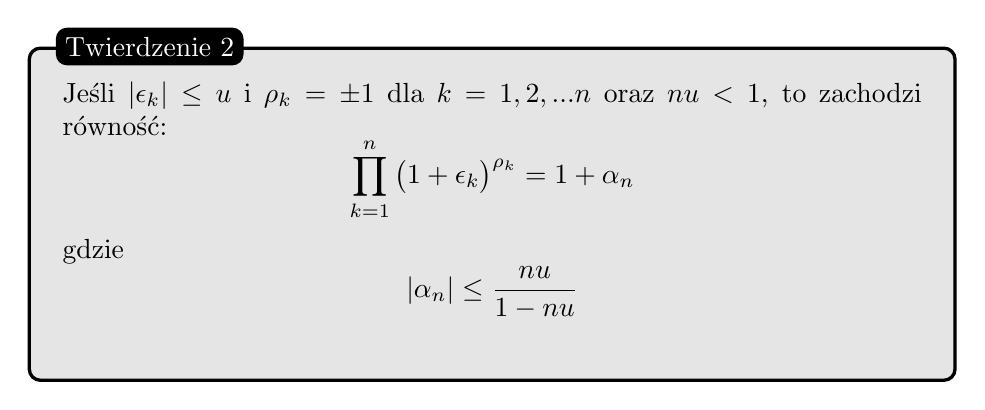
\begin{tikzpicture}
\node [draw={black}, fill=black!10, very thick, rectangle, rounded corners, inner sep=12pt, inner ysep=12pt] (box){%
    \begin{minipage}{.9\textwidth}
	Jeśli $|\epsilon_{k}| \leq u $ i  $\rho_{k} = \pm 1$ dla $k = 1,2,...n$ oraz $nu < 1$, to zachodzi równość:
	\[ \prod_{k=1}^{n}\big(1 + \epsilon_{k} \big) ^ {\rho_{k}} = 1 + \alpha_{n}\]
	gdzie \[ |\alpha_{n}|  \leq \frac{nu}{1-nu}\] 
\begin{large}
\end{large}	   


    
    \end{minipage}
};
\node[fill={black}, text=white, rounded corners, right=10pt] at (box.north west) {Twierdzenie 2};
\end{tikzpicture}
\end{center}





Chcemy dodać do siebie $n$ wyrazów ciągu. Dla uogólnienia nazwijmy je $ a_{1}, a_{2}, ... , a_{n}$.
 \[ \sum_{k=0}^n a_{k} = a_{1} + a_{2} + ... + a_{n}\] 
W komputerze powyższa suma obliczy się do:
\[  fl \bigg( \sum_{k=0}^n a_{k} \bigg) = fl\bigg( a_{1} + a_{2} + ... + a_{n} \bigg) = \big(\big(...\big(\big(a_{1} + a_{2}\big)\big(1+\epsilon_{2}\big) + a_{3}\big)\big(1+\epsilon_{3}\big)...\big) +a_{n}\big)\big(1+\epsilon_{n}\big) \] 
\[ = \;a_{1}\prod_{k=1}^{n} \big( 1+\epsilon_{k} \big) + a_{2}\prod_{k=2}^{n} \big( 1+\epsilon_{k} \big) +...+a_{n}\prod_{k=n}^{n} \big( 1+\epsilon_{k} \big) = \sum_{i=1}^{n} \bigg( a_{i} \prod_{k=i}^{n} \big( 1+\epsilon_{k} \big) \bigg) \;\;  \textrm{gdzie} \;\;\;  |\epsilon_{k}| \leq u \;\;\textrm{dla} \;\ k=2,3,...,n\]
\newpage
Oczywiście $\epsilon_{1} = 0$. Podstawmy: \[\prod_{k=i}^{n} \big( 1+\epsilon_{k} \big) = 1 + \alpha_{i} \]
Otrzymujemy: 
\[ fl(\sum_{i=1}^{n} a_{i})=\sum_{i=1}^{n} a_{i} \big(1 + \alpha_{i} \big) \] 
Wtedy z Twierdzenia 2 otrzymujemy, że:

\[ |\alpha_{i}| \leq \frac{(n+1-i)u}{1-(n+1-i)u} \;\; \textrm{gdzie} \;\;i=2,3,...n\]
Wywnioskować można stąd, że największe zaburzenie będzie występowało dla pierwszego składnika, analogicznie najmniejsze dla ostatniego.
\\\\
Spójrzmy teraz na poniższe sumy:
\[ 4\sum_{k=0}^{n} \frac{(-1)^{k}}{2k+1} \;\;\;\;\;\textrm{oraz} \;\;\;\;\;\; 4\sum_{k=n}^{0} \frac{(-1)^{k}}{2k+1}.\]
Różnią się one tylko kolejnością sumowania składników. \\Korzystając z powyższych obserwacji możemy się spodziewać, że w komputerze dokładniejszym wynikiem będzie suma druga. Będzie tak, z uwagi na to, że największy błąd będzie występował podczas sumowania dwóch najmnijeszych liczb sumy, analogicznie z kolejnymi błędami.


\section{Opis eksperymentu i wyniki}

Obliczenia zostały wykonane w języku Julia (wersja 1.5.2.)
przy użyciu 32-bitowej arytmetyki (32 bity przeznaczone na reprezentację mantysy).

Funkcje \textit{suma \textunderscore rosnaca(n)} oraz \textit{suma\textunderscore malejaca(n)} zostały uruchomione dla różnych wartości $n$,
a następnie została porównana precyzja, z jaką przybliżają liczbę $\pi$ poprzez porównanie wyniku
do wbudowanej stałej \texttt{MathConstants.pi}. 

Obliczona została liczba cyfr znaczących oraz iloraz błędów
każdego przybliżenia przy użyciu wzoru
\[\lfloor - log_{10}(\delta_{\pi})\rfloor \] gdzie
\[\delta_{\pi} = |\frac{\Delta \pi}{\pi}| \;\; \textrm{i}
\;\; \Delta \pi = \pi - \widetilde{\pi} \;\; \textrm{gdzie} \;\;
\widetilde{\pi} \;\; \textrm{oznacza otrzymane przybliżenie}\;\; \pi.\]

\subsection{Wyniki obliczeń oraz ich analiza}


\begin{center}
\includegraphics[scale=0.6]{plot1.png}
\\
\small{Rysunek 1: Wykres przedstawiający wyniki funkcji \textit{suma \textunderscore rosnaca(n)} dla $n = 10^1, 10^2, ..., 10^{7}$}

\includegraphics[scale=0.6]{plot2.png}
\\
\small{Rysunek 2: Wykres przedstawiający wyniki funkcji \textit{suma \textunderscore rosnaca(n)} oraz \textit{suma \textunderscore malejaca(n)}}
\newline
\newline
\newline
\end{center}
Zauważmy, że powyższe wykresy są tak do siebie podobne, że nie możemy  określić różnicy między nimi. Spójrzmy więc na wykres ilorazów błędów wspomnianych wyżej funkcji.\newline \newline

\begin{center}

\includegraphics[scale=0.6]{plot3.png}

\small{Rysunek 3: Wykres przedstawiający iloraz błędów funkcji \textit{suma \textunderscore rosnaca(n)} oraz \textit{suma \textunderscore rosnaca(n)},\\
\normalsize{$ |\frac{\delta_{\pi_{1}}}{\delta_{\pi_{1}}}|$ dla $n = 10^1,10^2,...,10^7 $} }

\end{center}


\begin{table}
\centering
\begin{tabular}{|c|c|c|c|}
    \hline
\large $n$ & \large $\lfloor - log_{10}(\delta_{\pi})\rfloor$  & $\delta_{\pi_{1}} = |\frac{\Delta \pi}{\pi}|$ & $\delta_{\pi_{2}} = |\frac{\Delta \pi}{\pi}|$
    \normalsize\\
    \hline
    $10^1$    & 1  & $\!\!\!\!\!0.028$ & $\!\!\!\!\!0.028$\\ \hline
    $10^2$    & 2  &   $\!\!0.0031$ & $\!\!0.0031$\\ \hline
    $10^3$    & 3  &  0.00031& 0.00031\\ \hline
    $10^4$    & 4  &  $\;\;\;\;3.17 \cdot 10^{-5}$& $\;\;\;\;3.17 \cdot 10^{-5}$\\ \hline
    $10^5$    & 5  &  $\;\;\;\;3.13 \cdot 10^{-6}$&$\;\;\;\;3.15 \cdot 10^{-6}$\\ \hline
    $10^6$    & 6  &  $\;\;\;\;2.72 \cdot 10^{-7}$ &$\;\;\;\;2.90 \cdot 10^{-7}$\\ \hline
    $10^7$    & 8  &   $\;\;\;\;8.24 \cdot 10^{-9}$ & $\;\;\;\;4.01 \cdot 10^{-9}$\\\hline

\end{tabular}
\center{Tablica 1: Wyniki programu dla wybranych wartości $n$.}
\end{table}

\begin{flushleft}
Jak widać błędy funkcji dla $ n = 10^1, 10^2, ... , 10^6$ są bardzo podobne. Zauważmy, że dla $n = 10^7$ iloraz błędów funkcji jest równy $ |\frac{\delta_{\pi_{1}}}{\delta_{\pi_{2}}}| \approx 2.1 $, wtedy funkcja \textit{suma \textunderscore rosnaca(n)} przybliża liczbę $\pi$ z dokładnością dwukrotnie mniejszą niż funkcja \textit{suma \textunderscore malejaca(n)}. \\Powyższe obserwacje potwierdzają naszą hipoteze - dokładniejszy wynik otrzymamy sumując sumę  $ 4\sum_{k=n}^{0} \frac{(-1)^{k}}{2k+1}$ w porządku odwrotnym.

\end{flushleft}







\end{document}